\documentclass[a4paper,12pt]{article}
%%% Default imports
\usepackage{listings} % Code listings
\usepackage{graphicx} % Images
\usepackage{booktabs} % Better tables
\usepackage{makecell}
\usepackage{enumitem} % Lists
\usepackage{dsfont}
\usepackage{geometry} % Page geometry
\usepackage[utf8]{inputenc} % Encoding
\usepackage[T2A]{fontenc} % Font
\usepackage[english, russian]{babel} % Multi-language support
\usepackage{titling} % Better titles
\usepackage{textcomp} % Old-style numbers? Check difference
\usepackage{mathtext} % Russian text in math expressions? Check difference
\usepackage{amsmath, amsfonts, amssymb, amsthm, mathtools} % Mathematics
\usepackage{bm} % Bold math symbols
\usepackage{icomma} % Better comma in numbers within math mode
\usepackage{xifthen} % Better if-expressions
\usepackage{transparent} % Transparent colors
\usepackage{caption}    % }
\usepackage{subcaption} % } Captioning figures
\usepackage[table,xcdraw]{xcolor} % Colors
\usepackage{textpos} % Absolute positioning
\usepackage{upgreek} % Cool greek letters

\usepackage{fancyvrb}
\usepackage{fvextra}
\usepackage{chngcntr}

%%% Page geometry
\setlength\parindent{0pt} % No indentation between paragraphs
\setlist{noitemsep} % No spacing between list items

\usepackage{float}
\usepackage{multirow}

\geometry{
    paper=a4paper,
    top=2.5cm,
    bottom=3cm,
    left=2.5cm,
    right=2.5cm,
    headheight=0.75cm,
    footskip=1.5cm,
    headsep=0.75cm,
}

%%% Numeration
\newcommand{\RNumb}[1]{\uppercase\expandafter{\romannumeral #1\relax}}
\newcommand{\thesec}{\arabic{section}}
\renewcommand\thesection{\arabic{section}}
\renewcommand\thesubsection{\thesection.\arabic{subsection}}
\renewcommand\thesubsubsection{\RNumb{\arabic{subsubsection}}}
\renewcommand{\sectionmark}[1]{\markright{\thesection\ #1}}
\renewcommand{\bf}{\textbf}
\renewcommand{\it}{\textit}
\def\hash{\texttt{\#}}
\def\cpp{\C\texttt{++}}

\counterwithin{figure}{section}
\counterwithin{table}{section}
\renewenvironment{titlepage}{\thispagestyle{empty}} % Include titlepage into page numeration

%%% Headers and footers
\usepackage{setspace}
\usepackage{fancyhdr}
\usepackage{lastpage}


%%% Graphics
% Custom colors
\definecolor{myblue}{RGB}{72, 184, 178}
\definecolor{myblue1}{RGB}{0, 109, 167}
\definecolor{commentgreen}{RGB}{2,112,10}
\definecolor{mauve}{rgb}{0.58,0,0.82}
\definecolor{amethyst}{RGB}{153, 102, 203}

\usepackage{pgfplots} % Plots
\usepackage{tikz}
\usetikzlibrary{3d,perspective,decorations.text}
\usetikzlibrary{animations}
\usetikzlibrary{positioning}
\usetikzlibrary{matrix}
\usepackage{tikz-cd}
\usetikzlibrary{cd}
\usetikzlibrary{karnaugh}
\pgfplotsset{width=6cm,compat=newest}
\usepackage{color}

\usepackage[framemethod=TikZ]{mdframed}
\newcommand{\definebox}[2]{\newcounter{#1}\newenvironment{#1}[1][]{\stepcounter{#1}\mdfsetup{frametitle={\tikz[baseline=(current bounding box.east),outer sep=0pt]\node[anchor=east,rectangle,fill=white]{\strut \MakeUppercase#1~\csname the#1\endcsname\ifstrempty{##1}{}{:~##1}};}}\mdfsetup{innertopmargin=1pt,linecolor=#2,linewidth=3pt,topline=true,frametitleaboveskip=\dimexpr-\ht\strutbox\relax,}\begin{mdframed}[]\relax}{\end{mdframed}}}
\definebox{definition}{black!90}
\definebox{theorem}{myblue1!90}
\definebox{demonstration}{amethyst!90}

\newcounter{Theorem}
\def\themytheorem{\thesection.\arabic{Theorem}}
\usepackage[most]{tcolorbox}
\tcbuselibrary{theorems}
\newtcbtheorem{Theorem}{Theorem}
{colframe=myblue!90,coltitle=black,colback=white,fonttitle=\bfseries}{Th}

%%% Code listings
\usepackage{matlab-prettifier}

\lstdefinestyle{cpp} {
    language=C++,
    frame=tb,
    tabsize=4,
    showstringspaces=false,
    numbers=left,
    captionpos=b,
    columns=flexible,
    upquote=true,
    commentstyle=\color{commentgreen},
    keywordstyle=\color{blue},
    stringstyle=\color{commentgreen},
    basicstyle=\small\ttfamily,
    emph={int,char,double,float,unsigned,void,bool,size\_t},
    emphstyle={\color{blue}},
    escapechar=\&,
    classoffset=1,
    otherkeywords={>,<,.,;,-,!,=,~},
    morekeywords={>,<,.,;,-,!,=,~},
    keywordstyle=\color{black},
    classoffset=0,
}
\lstdefinestyle{def} {
    frame=tb,
    tabsize=4,
    showstringspaces=false,
    numbers=left,
    captionpos=b,
    columns=flexible,
    upquote=true,
    commentstyle=\color{black},
    keywordstyle=\color{black},
    stringstyle=\color{black},
    basicstyle=\small\ttfamily,
    emph={int,char,double,float,unsigned,void,bool,size\_t},
    emphstyle={\color{black}},
    escapechar=\&,
    classoffset=1,
    otherkeywords={>,<,.,;,-,!,=,~},
    morekeywords={>,<,.,;,-,!,=,~},
    keywordstyle=\color{black},
    classoffset=0,
}
\lstdefinelanguage[RISC-V]{Assembler}
{
    alsoletter={.}, % allow dots in keywords
    alsodigit={0x}, % hex numbers are numbers too!
    morekeywords=[1]{ % instructions
    lb, lh, lw, lbu, lhu,
    sb, sh, sw,
    sll, slli, srl, srli, sra, srai,
    add, addi, sub, lui, auipc,
    xor, xori, or, ori, and, andi,
    slt, slti, sltu, sltiu,
    beq, bne, blt, bge, bltu, bgeu,
    j, jr, jal, jalr, ret,
    scall, break, nop
},
    morekeywords=[2]{ % sections of our code and other directives
    .align, .ascii, .asciiz, .byte, .data, .double, .extern,
    .float, .globl, .half, .kdata, .ktext, .set, .space, .text, .word
},
    morekeywords=[3]{ % registers
    zero, ra, sp, gp, tp, s0, fp,
    t0, t1, t2, t3, t4, t5, t6,
    s1, s2, s3, s4, s5, s6, s7, s8, s9, s10, s11,
    a0, a1, a2, a3, a4, a5, a6, a7,
    ft0, ft1, ft2, ft3, ft4, ft5, ft6, ft7,
    fs0, fs1, fs2, fs3, fs4, fs5, fs6, fs7, fs8, fs9, fs10, fs11,
    fa0, fa1, fa2, fa3, fa4, fa5, fa6, fa7
},
    morecomment=[l]{;},   % mark ; as line comment start
    morecomment=[l]{\#},  % as well as # (even though it is unconventional)
    morestring=[b]",      % mark " as string start/end
    morestring=[b]'       % also mark ' as string start/end
}
\lstdefinestyle{riscv} {
    basicstyle=\small\ttfamily,                    % very small code
    breaklines=true,                              % break long lines
    commentstyle=\itshape\color{green!50!black},  % comments are green
    keywordstyle=[1]\color{blue!80!black},        % instructions are blue
    keywordstyle=[2]\color{orange!80!black},      % sections/other directives are orange
    keywordstyle=[3]\color{red!50!black},         % registers are red
    stringstyle=\color{mauve},                    % strings are from the telekom
    identifierstyle=\color{teal},                 % user declared addresses are teal
    frame=l,                                      % black line on the left side of code
    captionpos=b,
    language=[RISC-V]Assembler,                   % all code is RISC-V
    tabsize=4,                                    % indent tabs with 4 spaces
    showstringspaces=false                        % do not replace spaces with weird underlines
}

%%% Other
\usepackage[normalem]{ulem} % }
\useunder{\uline}{\ul}{}    % } Underline text
\usepackage[colorlinks,urlcolor=blue,filecolor=blue,citecolor=blue,linkcolor = blue,unicode=true]{hyperref}
\usepackage{titlesec}
\titlelabel{\thetitle.\quad}
\usepackage{secdot}
\sectiondot{subsection}
\usepackage{kvmap} % Karnaugh-maps for logic functions
\usepackage{}
\newcommand{\projectname}[3]{
    \begin{center}
        \Large
        \textbf{#1}\\[10pt]
        \textbf{#2}\\[10pt]
        \normalsize
        #3
        \rule{\linewidth}{0.4pt}
    \end{center}
}

\newcommand{\hfconfiguration}[3]{
    \pagestyle{fancy}
    \fancyhead[LE,RO]{}
    \fancyhead[LO,RE]{#1}
    \renewcommand{\footrulewidth}{0.4pt}
    \fancyfoot[C]{\thepage/\pageref*{LastPage}}
    \fancyfoot[LO,RE]{#2}
    \fancyfoot[LE,RO]{#3}
}

\newcommand{\filename}[2]{
    \pagebreak
    \titleformat{\section}
    [display]
    {\bfseries\Large}
    {}
    {0ex}
    {
        \vspace{-4.5ex}
        % \rule{\textwidth}{1pt}
        #1 \centering
    % \vspace{1ex}
    }
    [
        \normalfont\large
        #2
        \rule{\textwidth}{0.4pt}
        \normalsize
    ]
}

\newcommand{\project}[6]{
    \projectname{#1}{#2}{#3}
    \pagestyle{empty}
    \tableofcontents
    \newpage
    \hfconfiguration{#4}{#5}{#6}
}
%%% Final touch
\usepackage{subfiles}


\begin{document}
    \begin{titlepage}
    \begin{center}
        \large Санкт-Петербургский политехнический университет Петра Великого\\
        \large Институт компьютерных наук и технологий \\
        \large Кафедра компьютерных систем и программных технологий\\[6cm]


        \huge Расчетная работа №2\\[0.5cm]
        \large по дисциплине <<Теория вероятностей и математическая статистика>>\\[0.1cm]
        \large\textbf{}\\[5cm]
    \end{center}


    \begin{flushright}
        \begin{minipage}{0.25\textwidth}
            \begin{flushleft}

                \large\textbf{Работу выполнил:}\\
                \large Ильин В.П.\\
                \large {Группа:} 35300901/10005\\

                \large \textbf{Преподаватель:}\\
                \large Куляшова З.В.

            \end{flushleft}
        \end{minipage}
    \end{flushright}

    \vfill

    \begin{center}
        \large Санкт-Петербург\\
        \large \the\year
    \end{center}
\end{titlepage}

\vfill
\newpage
    \hfconfiguration{Расчетная работа №2}{}{}    

    \section{Оценка полных характеристик распределения}
    Рассмотрим вывод \texttt{part1.py}:
    \begin{figure}[H]
        \centering
        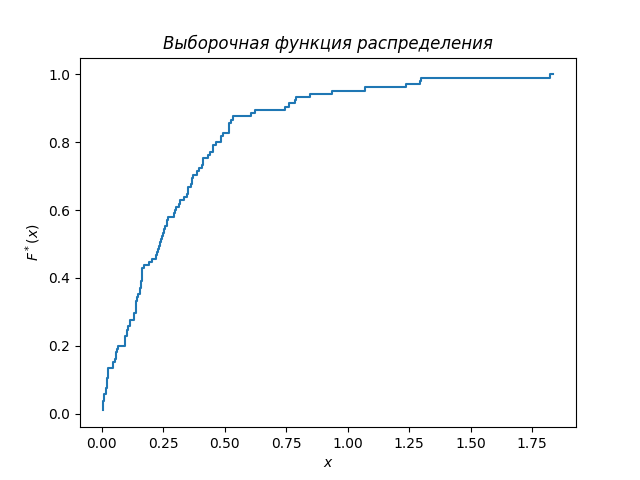
\includegraphics[width=0.7\linewidth]{polytech/stats/homework-2/subfiles/fig/1}
        \caption{Выборочная функция распределения}
    \end{figure}
    \begin{figure}[H]
        \centering
        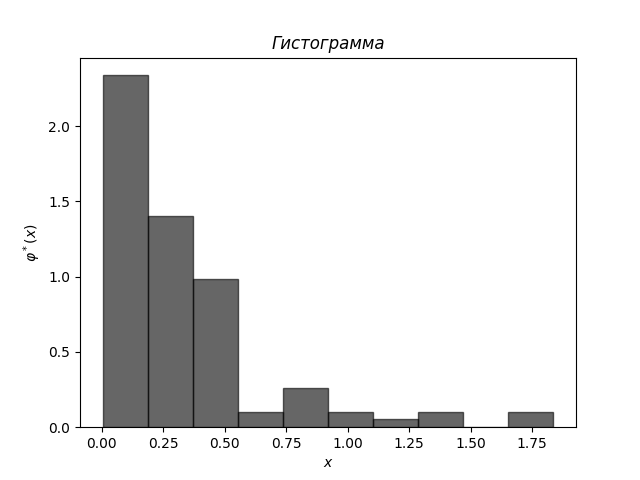
\includegraphics[width=0.7\linewidth]{polytech/stats/homework-2/subfiles/fig/2}
        \caption{Гистограмма $\varphi^*(x)$}
    \end{figure}
    \section{Частные характеристики распределения}
    Будем искать характеристики для двух выборок: помимо полной, выделим
    ее подпоследовательность длиной 20. Найдем точечные оценки (\texttt{part21.py}):
    \begin{enumerate}
        \item Полная выборка
        \begin{itemize}
            \item Выборочное среднее $= 0.3326$
            \item Выборочная медиана $= 0.2392$
            \item Середина размаха $= 0.91975$
            \item Второй центральный момент (дисперсия) $= 0.1198$
            \item Третий центральный момент $= 0.092$
            \item Четвертый центральный момент $= 0.1269$
            \item Коэффициент асимметрии $=2.2181$
            \item Коэффициент эксцесса $= 5.8456$
            \item Границы интерквантильного промежутка (для $P = 0.95$): $[-0.3641, 0.9111]$
        \end{itemize}
        \item Частичная выборка
        \begin{itemize}
            \item Выборочное среднее $= 0.336$
            \item Выборочная медиана $= 0.2364$
            \item Середина размаха $= 0.6802$
            \item Второй центральный момент (дисперсия) $= 0.0841$
            \item Третий центральный момент $= 0.0493$
            \item Четвертый центральный момент $= 0.0472$
            \item Коэффициент асимметрии $=2.0238$
            \item Коэффициент эксцесса $= 3.6748$
        \end{itemize}
    \end{enumerate}
    Интервальные оценки с доверительной вероятностью $Q = 0.95$:
    \begin{enumerate}
        \item Полная выборка
        \begin{itemize}
            \item Первый начальный момент $= 0.3326$
            \item Интервальные оценки для первого начального момента: $(0.2653, 0.3999)$
            \item Второй центральный момент $= 0.1209$
            \item Интервальные оценки для второго центрального момента: $(0.0938, 0.1619)$
            \item Интерквантильный промежуток (параметрический подход): $(0.257, 0.408)$
            \item Интерквантильный промежуток (непараметрический подход): $(0.232, 0.251)$
        \end{itemize}
        \item Частичная выборка
        \begin{itemize}
            \item Первый начальный момент $= 0.4596$
            \item Интервальные оценки для первого начального момента: $(0.2144, 0.7047)$
            \item Второй центральный момент $= 0.2744$
            \item Интервальные оценки для второго центрального момента: $(0.1587, 0.5854)$
        \end{itemize}
    \end{enumerate}
    
    \section{Идентификация закона распределения генеральной совокупности}
    Исходя из вида гистограммы, можно сделать предположение об экспоненциальном
    виде закона распределения.
    \begin{figure}[H]
        \centering
        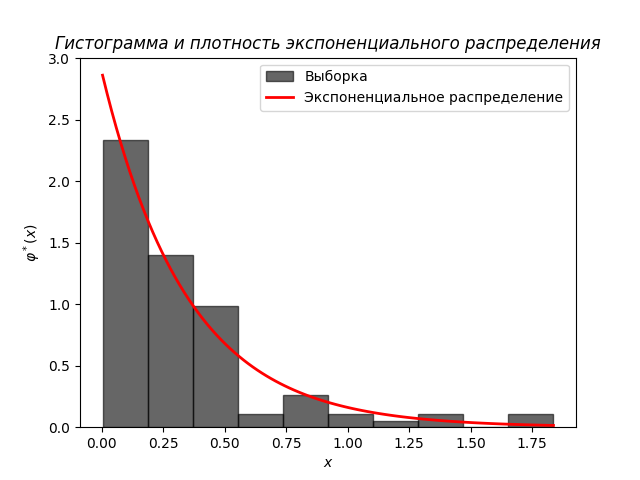
\includegraphics[width=0.7\linewidth]{polytech/stats/homework-2/subfiles/fig/3}
    \end{figure}
    Проверим гипотезу несколькими критериями (\texttt{part3.py}):
    \begin{enumerate}
        \item Критерий <<Хи-квадрат>>: подходит;
        \item Критерий типа Колмогорова-Смирного: подходит;
        \item Критерий <<Омега-квадрат>> Мизеса: подходит.
    \end{enumerate}

    \section{Вывод}
    В ходе работы были оценены полные и частные характеристики распределения данной случайной величины.
    Было идентифицировано, что она подчиняется экспоненциальному закону распределения.
    \newpage
    \section*{Приложение 1}
    % \lstinputlisting[style=py, caption={main.py}, captionpos=b, label={lst:main}]{polytech/stats/homework-2/subfiles/main.py}
    % \lstinputlisting[style=py, caption={part1.py}, captionpos=b, label={lst:part1}]{polytech/stats/homework-2/subfiles/part1.py}
    % \lstinputlisting[style=py, caption={part21.py}, captionpos=b, label={lst:part21}]{polytech/stats/homework-2/subfiles/part21.py}
    % \lstinputlisting[style=py, caption={part23.py}, captionpos=b, label={lst:part23}]{polytech/stats/homework-2/subfiles/part23.py}
    % \lstinputlisting[style=py, caption={part3.py}, captionpos=b, label={lst:part3}]{polytech/stats/homework-2/subfiles/part3.py}
    \begin{figure}[H]
        \centering
        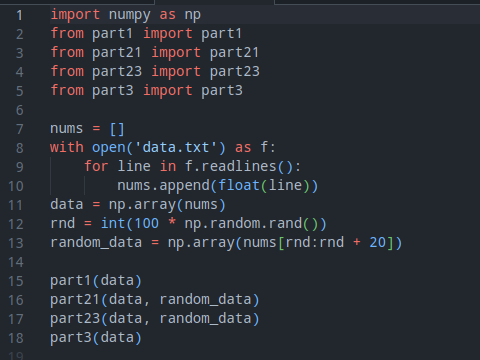
\includegraphics[width=0.65\linewidth]{polytech/stats/homework-2/subfiles/fig/main}
        \caption{\texttt{main.py}}
    \end{figure}
    \begin{figure}[H]
        \centering
        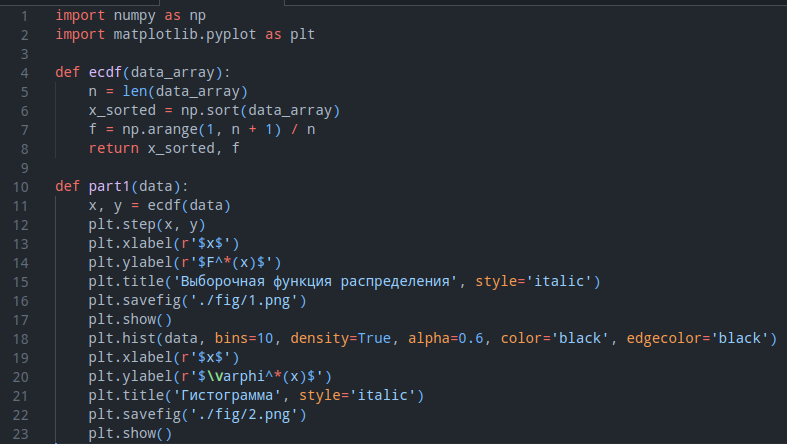
\includegraphics[width=0.7\linewidth]{polytech/stats/homework-2/subfiles/fig/part1}
        \caption{\texttt{part1.py}}
    \end{figure}
    \begin{figure}[H]
        \centering
        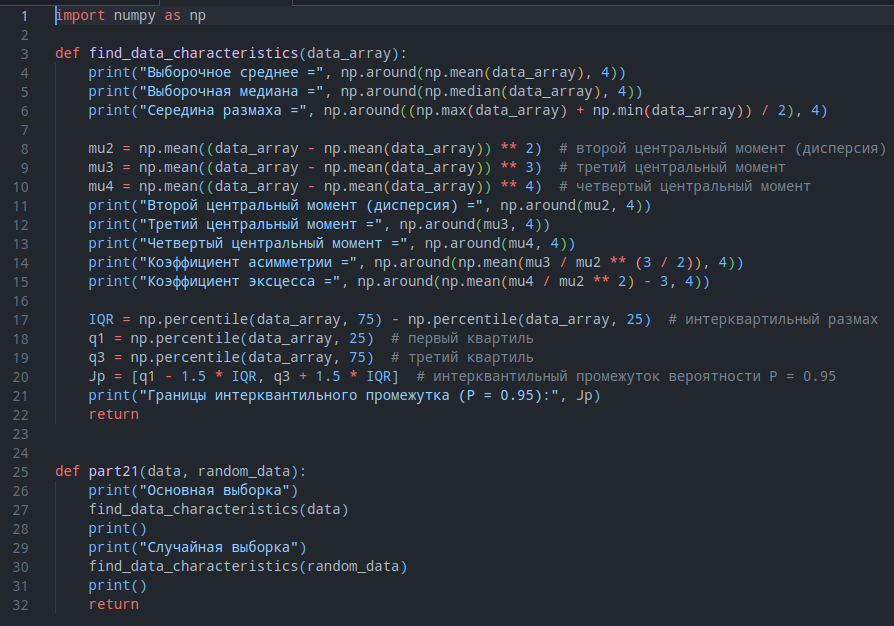
\includegraphics[width=\linewidth]{polytech/stats/homework-2/subfiles/fig/part21}
        \caption{\texttt{part21.py}}
    \end{figure}
    \begin{figure}[H]
        \centering
        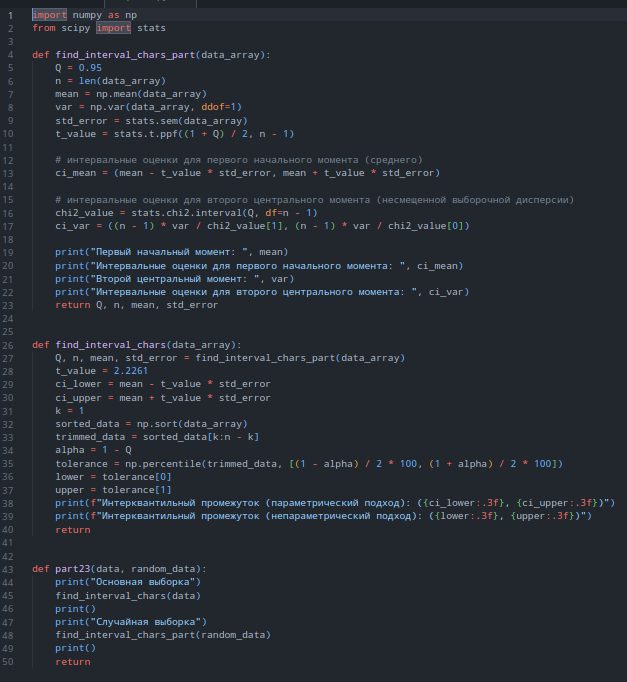
\includegraphics[width=\linewidth]{polytech/stats/homework-2/subfiles/fig/part22}
        \caption{\texttt{part23.py}}
    \end{figure}
    \begin{figure}[H]
        \centering
        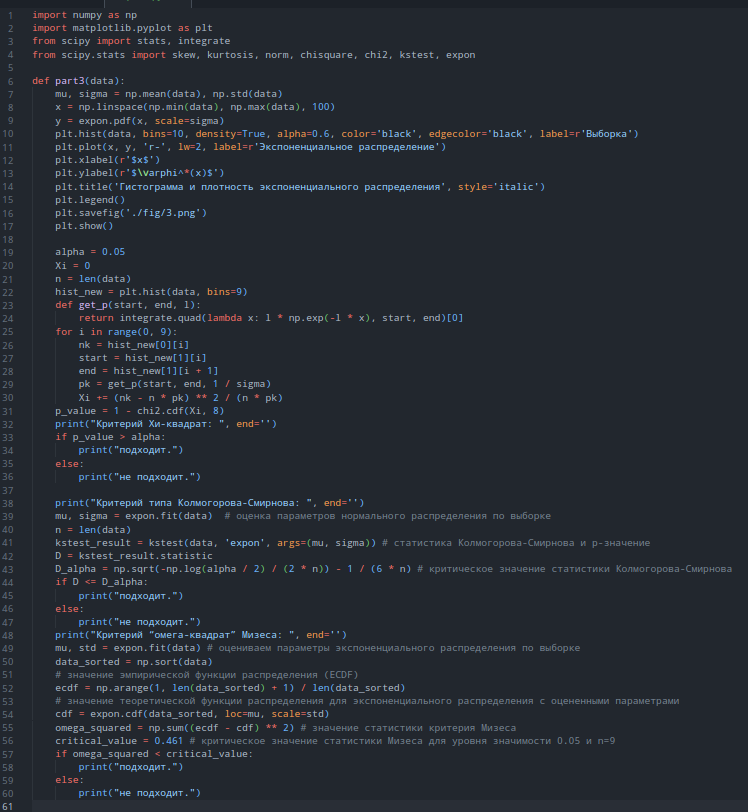
\includegraphics[width=\linewidth]{polytech/stats/homework-2/subfiles/fig/part3}
        \caption{\texttt{part3.py}}
    \end{figure}
\end{document}
